\documentclass{beamer}
\usetheme{default}
\usepackage{lmodern}
\usepackage{amsmath}
\usepackage{amssymb}
\usepackage{proof}
\usepackage{parskip}
\usepackage{wasysym}
\usepackage{hyperref}
\usepackage{verbatim}
\usepackage{relsize}
\usepackage[T1]{fontenc}

\hypersetup{
  colorlinks=true,
  urlcolor=blue
}

\newcommand{\hl}[1]{\color{red}{#1}}
\newcommand{\arr}[1]{\ensuremath\xrightarrow{#1}}

\title{Generating code in a term rewriting framework}
\author{Geoffrey C. Hulette}
\date{\today}

\begin{document}

\begin{frame}[plain]
  \titlepage
\end{frame}


%%
\begin{frame}{About me}

I am currently a Ph.D. student in computer science at the University of
Oregon, and also a Sandia intern. 

My research interests include:

\begin{itemize}

\item Programming language theory and formal semantics;

\item Tradeoffs between the expressive power of formal systems and automated
reasoning about them;

\item Methods for ensuring programs are correct by construction (e.g. type
systems, automated theorem proving, code generation).

\end{itemize}

These interests intersect in the field of \emph{formal methods}.

\end{frame}


%%
\begin{frame}{Twig}

My dissertation research has focused on the design of a formal system for code
generation called \textbf{Twig}.

Twig's semantics are based on the theory of term rewriting, which is important
for reasoning about equivalence relationships. This is an important problem in
formal methods.

\end{frame}


%%
\begin{frame}{Outline}

Today I will be talking about:

\begin{enumerate}
  \item Why generating code for GPUs is difficult
  \item Term rewriting theory
  \item System S
  \item How Twig generates code
  \item How Twig generates GPU code
  \item Connections to formal methods
\end{enumerate}

\end{frame}


%%
\begin{frame}{Problem: Programming GPUs}

Writing code for GPUs is tedious. In OpenCL, a simple vector operation
requires more than 200 LOC.

One solution is to use a higher-level representation for GPU programs, and
generate the low-level CUDA or OpenCL code.

\end{frame}


%%
\begin{frame}{Problem: Programming GPUs}

Na\"ive GPU code generation may produce inefficient code.

\begin{itemize}

\item Generated code must be generic enough to support different data types
and operations. Supporting this capability at runtime may introduce complex
conditional branching.

\item High-level representations of GPU operations should abstract
``book-keeping'' operations (e.g. moving data to and from the device). To
avoid generating redundant code we need to compose abstractions intelligently.

\end{itemize}

\end{frame}


%%
\begin{frame}{Our approach}

Our solution is \textbf{Twig}, a language for code generation that features:

\begin{itemize}

\item \textbf{Type-directed code generation} to minimize runtime overhead;

\item Simple but effective \textbf{algebraic manipulation} of Twig
expressions, which can eliminate redundant operations.

\end{itemize}

\end{frame}


%%
\begin{frame}{Our approach}

\textbf{Twig}, is based on the theory of \emph{term rewriting}.

Next, we cover some basic definitions and results from that theory.

\end{frame}


%%
\begin{frame}{Term Rewriting}

\textbf{Term rewriting} is an approach to programming that is well-suited to
code generation. The formalism is based on abstract reduction theory and
universal algebra.

The key idea is to write a program as a set of transformative \emph{rules}
which are applied sequentially to transform inputs to outputs.

\end{frame}


%%
\begin{frame}{Preview}

In Twig, we will use rules that transform \emph{types} in the target language
(i.e. C), and which generate code as a side-effect of application.

\end{frame}


%%
\begin{frame}{Abstract reduction}

\textbf{Reduction} abstracts and formalizes the idea of step-by-step
transformation. An \textbf{abstract reduction system} is a pair $(A,\to)$
where $\to$ is a binary relation on $A$.

Some terminology:

\begin{itemize}
  \item $x \in A$ is \textbf{reducible} iff $\exists y \in A$ s.t. $ x \to y$;
  \item $x \in A$ is in \textbf{normal form} if $x$ is not reducible.
\end{itemize}

\end{frame}


%%
\begin{frame}{Equivalence}

If we regard $\to$ as \textbf{identities}, we can ask whether any two objects
in $A$ are \textbf{equivalent}.

\begin{center}
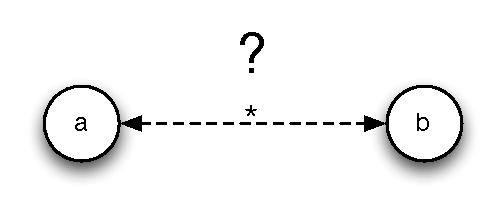
\includegraphics[width=2in]{images/equivalence}
\end{center}

\end{frame}


%%
\begin{frame}{Equivalence}

Deciding equivalence via an undirected search will (probably) be inefficient.

Instead, we can reduce objects to a normal form. If two objects have identical
normal forms, we say they are equivalent.

\begin{center}
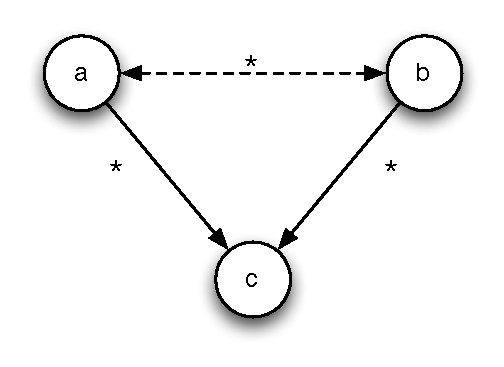
\includegraphics[width=2in]{images/church-rosser}
\end{center}

\end{frame}


%%
\begin{frame}{Equivalence}

Clearly, this approach works iff

\begin{itemize}
  \item reduction eventually \textbf{terminates} and
  \item normal forms are unique, i.e. the system is \textbf{confluent}.
\end{itemize}

\end{frame}


%%
\begin{frame}{Termination}

A reduction system \emph{terminates} iff there exists no infinite chain of
reduction steps, e.g.

\[
a_0 \to a_1 \to a_2 \to \ldots
\]

Naturally, proving termination is undecidable in general.

\end{frame}


%%
\begin{frame}{Termination}

Note that confluence does not entail termination:

\begin{center}
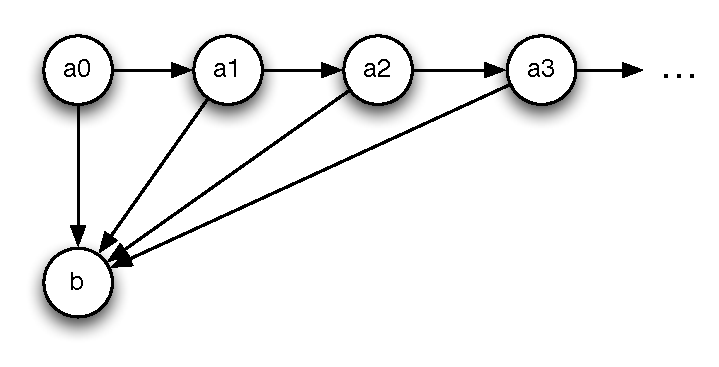
\includegraphics[width=2in]{images/ars}
\end{center}

\end{frame}


%%
\begin{frame}{Confluence}

Every object in a confluent system has at most one normal form. A reduction
system is \emph{confluent} iff

\[
\forall x,y_1,y_2 . 
x \xrightarrow{*} y_1 \land x \xrightarrow{*} y_2 \implies 
\exists z . y_1 \xrightarrow{*} z \land y_2 \xrightarrow{*} z
\]

\begin{center}
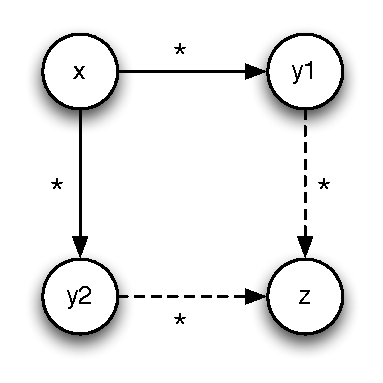
\includegraphics[width=1.5in]{images/confluence}
\end{center}

Determining whether a reduction system is confluent is undecidable in general,
but it is decidable for terminating systems.

\end{frame}


%%
\begin{frame}{Terms}

Informally, \emph{terms} are tree-structured data where labeled nodes
represent either \emph{constructors} having 0 or more sub-terms, or else
\emph{variables}.

Terminology:

\begin{itemize}
  \item Constructors with zero arguments are called \emph{constants};
  \item Terms with no variables are called \emph{ground} terms.
\end{itemize}

By (my own) convention, variable names begin with a capital letter, to
distinguish from constructors.

\end{frame}


%%
\begin{frame}{Term example}

The term \texttt{a(b,c(d))} can be represented:

\begin{center}
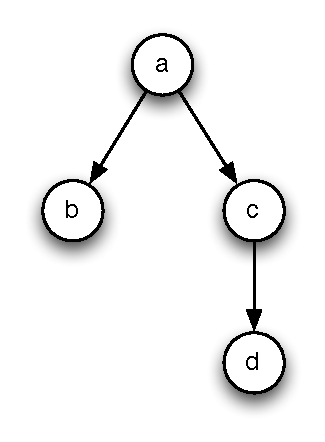
\includegraphics[height=1.5in]{images/example-term-1}
\end{center}

This is a ground term. The functions \texttt{b} and \texttt{d} are constants,
\texttt{c} is unary, and \texttt{a} is binary.

\end{frame}


%%
\begin{frame}{Term example}

The term \texttt{a(X,c(Y,d))} can be represented:

\begin{center}
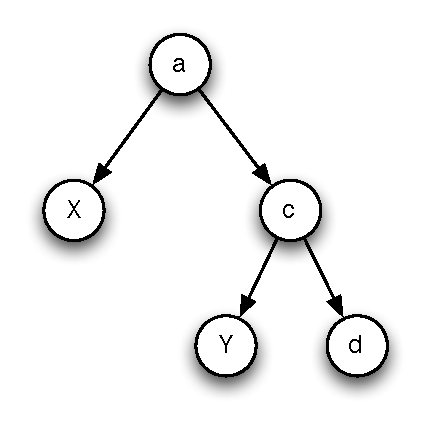
\includegraphics[height=1.5in]{images/example-term-2}
\end{center}

This is not a ground term, and its variables are \texttt{X} and \texttt{Y}.
Note that variables cannot have sub-terms.

\end{frame}


%%
\begin{frame}{Terms}

Slightly more formally, a set of constructors $\Sigma$ and a set of variables
$X$ determine a set of terms $T(\Sigma,X)$ iff $\Sigma \cap X = \emptyset$.

We refer to the ground terms as $T(\Sigma)$ and clearly $T(\Sigma) \subseteq
T(\Sigma,X)$.

\end{frame}


%%
\begin{frame}{Substitution}

A \textbf{ground-substitution} in $T(\Sigma,X)$ is a partial function $\sigma
: X \to T(\Sigma)$, i.e. from variables to ground terms in $T(\Sigma,X)$. We
use $\sigma$ to define a partial function $\delta : T(\Sigma,X) \to
T(\Sigma)$.

The application of $\delta$ to a term $t \in T(\Sigma,X)$ replaces the
variables in $t$ with the corresponding image of that variable under $\sigma$.
The result is a ground term $t' \in T(\Sigma)$. The result is undefined if $t$
contains a variable $x$ such that $\sigma(x)$ is undefined.

Substitutions $\sigma$ and $\tau$ can be composed such that for all $x \in X
\:.\: \sigma\tau(x) = t$ iff

\begin{itemize}
  \item $\sigma(x) = t$ and $\tau(x)$ is undefined or
  \item $\tau(x) = t$ and $\sigma(x)$ is undefined or
  \item $\sigma(x) = \tau(x) = t$
\end{itemize}

\end{frame}


%%
\begin{frame}{System S}

\textbf{System S} is a formal semantics for term rewriting systems. It is the
basis for Twig's rule expressions.

The key idea in System S is user-definable rewriting \textbf{strategies} --
i.e. methods for choosing which rule to apply in a given context.

\end{frame}


%%
\begin{frame}{System S: Primitive rules}

Term rewriting rules are written:

\begin{itemize}
  \item \texttt{[} $t_1$ \texttt{->} $t_2$ \texttt{]}
\end{itemize}

where $t_1$ and $t_2$ are terms. Given a set of ground terms $T$, a rule is a
function $r : T \to (T \cup \{\bot\})$.

\end{frame}


%%
\begin{frame}{System S: Primitive rules}

The result $\bot$ can be interpreted as ``failure'' or ``undefined.'' It is
returned in case:

\begin{itemize}
  \item The input term does not ``match'' $t_1$;
  \item $t_2$ contains variables not bound in $t_1$ (i.e. substitution is undefined).
\end{itemize}

\end{frame}


%%
\begin{frame}{System S: Primitive rule application}

Pseudo-code for rule application:

\verbatiminput{code/apply.hs}

\end{frame}


%%
\begin{frame}{System S: Primitive rule examples}

For example, here are De Morgan's laws:

\begin{itemize}
  \item \texttt{[not(or(P,Q)) -> and(not(P),not(Q))]}
  \item \texttt{[not(and(P,Q)) -> or(not(P),not(Q))]}
\end{itemize}

\end{frame}

%%
\begin{frame}{System S: Primitive rules}

Some things to note about rules in System S:

\begin{itemize}
  \item Rules are unidirectional
  \item Rules match using only the outermost constructor
  \item Matched variables need not be used\\
        e.g. \texttt{[or(true,P) -> true]}
  \item Matching is non-linear\\
        e.g. \texttt{[and(P,not(P)) -> false]}
\end{itemize}

\end{frame}


%%
\begin{frame}{System S: Basic combinators}

Sequence:

\[
\infer{t \arr{s_1;s_2} t''}{t \arr{s_1} t' \quad t' \arr{s_2} t''}
\qquad 
\infer{t \arr{s_1;s_2} \bot}{t \arr{s_1} \bot}
\qquad
\infer{t \arr{s_1;s_2} \bot}{t \arr{s_1} t' \quad t' \arr{s_2} \bot}
\]

Left-biased choice:

\[
\infer{t \arr{s_1|s_2} t'}{t \arr{s_1} t'}
\qquad 
\infer{t \arr{s_1|s_2} t'}{t \arr{s_1} \bot \quad t \arr{s_2} t'}
\qquad
\infer{t \arr{s_1|s_2} \bot}{t \arr{s_1} \bot \quad t \arr{s_2} \bot}
\]

\end{frame}


%%
\begin{frame}{System S: More basic combinators}

Constants:

\[
\infer{t \arr{\mathtt{id}} t}{}
\qquad
\infer{t \arr{\mathtt{fail}} \bot}{}
\]

Discard result:

\[
\infer{t \arr{?s} t}{t \arr{s} t'}
\qquad 
\infer{t \arr{?s} \bot}{t \arr{s} \bot}
\qquad
\infer{t \arr{\lnot s} \bot}{t \arr{s} t'}
\qquad 
\infer{t \arr{\lnot s} t}{t \arr{s} \bot}
\]

Fix-point:

\[
\infer{t \arr{\mu x(s)} t'}{t \arr{s[x := \mu x(s)]} t'}
\qquad 
\infer{t \arr{\mu x(s)} \bot}{t \arr{s[x := \mu x(s)]} \bot}
\]

\end{frame}


%%
\begin{frame}{Tuples}

Twig introduces special syntax for ``tuple'' terms:

\begin{itemize}
  \item ``\texttt{(}$t_1,t_2,\ldots,t_n$\texttt{)}'' 
        $:=$ \texttt{tuple(}$t_1,t_2,\ldots,t_n$\texttt{)}
\end{itemize}

and some tuple combinators.

All tuple combinators share these failure semantics:

\[
\infer{f(\ldots) \arr{s} \bot}
{f \neq \mathtt{tuple}}
\qquad
\infer{\mathtt{tuple}(t_1,\ldots,t_n) \arr{s(i)} \bot}{i > n}
\]

\end{frame}

%%
\begin{frame}{Tuple combinators}

Projection:

\[
\infer{\mathtt{tuple}(\ldots,t_i,\ldots) \arr{\#i} t_i}{}
\]

Path:

\[
\infer{\mathtt{tuple}(\ldots,t_i,\ldots) \arr{\#i(s)} 
\mathtt{tuple}(\ldots,t_i',\ldots)}
{t_i \arr{s} t_i'}
\]

\[
\infer{\mathtt{tuple}(\ldots,t_i,\ldots) \arr{\#i(s)} \bot}
{t_i \arr{s} \bot}
\]

\end{frame}


%%
\begin{frame}{Tuple combinators}

Congruence:

\[
\infer{
\mathtt{tuple}(t_1,\ldots,t_n)
\arr{(s_1,\ldots,s_n)}
\mathtt{tuple}(t_1',\ldots,t_n') }
{t_1 \arr{s_1} t_1' \quad \ldots \quad t_n \arr{s_n} t_n'}
\]

\[
\infer{
\mathtt{tuple}(\ldots,t_i,\ldots)
\arr{(\ldots,s_i,\ldots)}
\bot}
{t_i \arr{s_i} \bot}
\]

\end{frame}


%%
\begin{frame}{Tuple combinators}

Branch:

\[
\infer{
  t \arr{\mathtt{\#branch}(s_1,\ldots,s_n)}
  \mathtt{tuple}(t_1',\ldots,t_n')
}{t \arr{s_1} t_1' \quad \ldots \quad t \arr{s_n} t_n'}
\]

\[
\infer
{t \arr{\mathtt{\#branch}(\ldots,s_i,\dots)} \bot}
{t \arr{s_i} \bot}
\]

\end{frame}


%%
\begin{frame}{Tuple combinators}

Map:

\[
\infer{
  \mathtt{tuple}(t_1,\ldots,t_n)
  \arr{\mathtt{\#map}(s)}
  \mathtt{tuple}(t_1',\ldots,t_n')
}{t_1 \arr{s} t_1' \quad \ldots \quad t_n \arr{s} t_n'}
\]

\[
\infer
{\mathtt{tuple}(\ldots,t_i,\ldots) \arr{\mathtt{\#map}(s)} \bot}
{t_i \arr{s} \bot}
\]

\end{frame}


%%
\begin{frame}{System S: Properties}

A few things to notice about System S/Twig:

\begin{itemize}

\item Rules are always applied deterministically, therefore all Twig programs
are confluent.

\item Programs which do not involve the \texttt{Fix} combinator have finite
chains of rule application, therefore these programs terminate.

\end{itemize}

\end{frame}


%%
\begin{frame}{Values in Twig}

To generate code, we let terms range over types in a given target language.

Types in the target language are values in Twig.

\begin{center}
\begin{tabular}{c | c}
  Twig               & C \\
  \hline                       
  \texttt{int}       & \texttt{int}    \\
  \texttt{double}    & \texttt{double} \\
  \texttt{ptr(int)}  & \texttt{int*}   \\
  \texttt{ptr(char)} & \texttt{char*}  \\
\end{tabular}
\end{center}

\end{frame}


%%
\begin{frame}{Values in Twig}

Twig supports custom mapping between terms and types in the target language,
including application-specific types.

\begin{center}
\begin{tabular}{c | c}
  Twig                  & C \\
  \hline                       
  \texttt{string}       & \texttt{char*} \\
  \texttt{array2D(int)} & \texttt{int**} \\
  \texttt{complex}      & \texttt{struct complex \{double r; double i;\}} \\
\end{tabular}
\end{center}

\end{frame}


%%
\begin{frame}{Extended rules for code generation}

In Twig, code is generated as a side effect of rule evaluation. We extend the
semantics of primitive rules so that they are functions

\[
T \to (T \times M) \cup \{\bot\}
\]

where $M$ ranges over code \emph{templates} and include an ``empty'' template.

We also extend the semantics of the various combinators to correctly combine
templates according to a formal \emph{template algebra}.

\end{frame}


%%
\begin{frame}{Code templates}

Primitive rules have a syntax for attaching a templates, based on that of
SWIG.

\begin{itemize}
  \item \texttt{[int -> float] \{ \$out = (float)\$in; \}}
  \item \texttt{[string -> int] \{ \$out = atoi(\$in); \}}
\end{itemize}  

Twig takes care of declaring and naming the variables, and supports parameters
and temporary variables.

\end{frame}


%%
\begin{frame}[fragile]{Generating code from tuples}

Tuples represent a collection of values, and these may be accessed
individually within a template:

\begin{verbatim}
[(float,float) -> float] {
  $out = $in1 * $in1 + $in2 * $in2;
}
\end{verbatim}

Non-tuple sub-terms may not be accessed with this syntax, because there is no
generic way to decompose aggregate values.

\end{frame}


%%
\begin{frame}[fragile]{Generating code from tuples}

Variables in rules are fine, but it is up to the programmer to make sure that
the template makes sense.

\begin{verbatim}
[(X,X) -> X] {
  $out = $in1 * $in1 + $in2 * $in2;
}
\end{verbatim}

If done carefully (e.g. making sure that \texttt{X} is an \texttt{int},
\texttt{float}, etc. beforehand), this technique enables polymorphic code
generation.

\end{frame}


%%
\begin{frame}[fragile]{GPU Example revisited}

So now we can write our simple GPU example:

\small
\verbatiminput{code/gpu.twig}
\normalsize

\end{frame}


%%
\begin{frame}[fragile]{Algebraic manipulation}

Notice the \texttt{\@reduce} directive:

\begin{verbatim}
@reduce copyArrayFromGPU ; copyArrayToGPU => id
\end{verbatim}

This tells Twig to replace the expression

\texttt{copyArrayFromGPU ; copyArrayToGPU} 

with the identity rule wherever it occurs. The \texttt{@reduce} directive
allows for user-defined algebraic identities.

\end{frame}


%%
\begin{frame}[fragile]{Algebraic manipulation}

Twig provides many built-in identities, for example:

\begin{itemize}
  \item \texttt{id;X => X}
  \teim \texttt{X;fail => fail}
  \item \texttt{X;(Y|Z) => (X;Y)|(X;Z)}
  \item \texttt{\#all($r_1,\ldots,r_n$);\#all($s_1,\ldots,s_n$) => 
  \#all($r_1$;$s_1$,\ldots,$r_n$;$s_n$)}
  \item $\ldots$
\end{itemize}

These reductions are performed with a general-purpose rewrite engine, so it is
important that the set be confluent and terminating.

\end{frame}


%%
\begin{frame}[fragile]{Evaluation of Twig's Utility}

Twig has been (mostly) implemented in Haskell. I am in the process of
evaluating its application to the GPU problem.

\begin{itemize}

\item We have demonstrated Twig's algebraic reduction on simple GPU programs.

\item We are evaluating its effectiveness for large, realistic GPU programs.

\item We are comparing the code generated by Twig against other GPU code
generators such as PyCUDA.

\end{itemize}

\end{frame}


%%
\begin{frame}[fragile]{Other applications}

We are also using Twig to generate efficient multi-language bindings. Twig's
algebraic identities can be used to bypass intermediate interoperability
layers in certain contexts.

\begin{center}
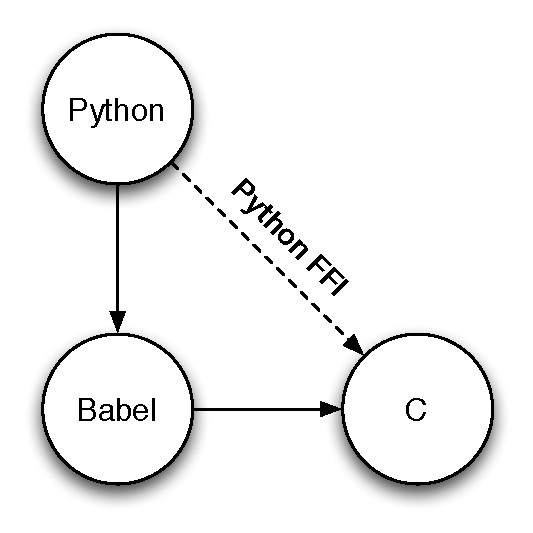
\includegraphics[height=1.5in]{images/multi-language}
\end{center}

\end{frame}


%%
\begin{frame}{Related work}

Twig began as a method for multi-language binding generation, influenced by
ad-hoc tools such as SWIG. SWIG is effective but basic. In particular, there
is no way to compose rules, and no way to generate code other than bindings.

Moby/FIG was a major influence on Twig. Twig is a more general tool than FIG,
but shares a similar formal approach.

PyCUDA generates native GPU code from Python. The Python GPU functions
generate C code, which is then compiled, evaluated, and returned back into
Python at runtime.

\end{frame}


%%
\begin{frame}{Future directions}

In the future Twig could be extended:

\begin{itemize}

\item Allowing users to generate code in other languages (e.g. Python).

\item Supporting more sophisticated code generation, e.g. functors.

\item Ensuring that user-defined reductions terminate and are confluent.

\end{itemize}

Twig belongs to a class of tools which are also useful for program analysis
and formal methods...

\end{frame}


%% 
\begin{frame}{Formal methods}

Term rewriting is fundamental in formal methods. It is relevant whenever you
need to reason about equivalence relationships. Proofs are a particularly
important example.

Formal semantics and type systems are also important tools for formal methods.

Automated reasoning about languages like C is difficult in general because
programs do not contain high-level semantic information.

Formal semantics can be used to augment general-purpose languages and enable
higher-level reasoning. Code generation in Twig is an example of this
approach.

These techniques help us build software that is correct by construction.

\end{frame}


%% 
\begin{frame}{Formal methods}

``Formal methods'' refers to several techniques for mathematical reasoning
about software properties. These include:

\begin{itemize}
  \item Model checking;
  \item Formal semantics;
  \item Type systems.
\end{itemize}

In general formal methods may be high-cost, but for domains like
cyber-security and NW they are often justified.

\end{frame}


%% 
\begin{frame}{Conclusion}

Questions?

My email: \texttt{ghulett@sandia.gov}

\end{frame}


\end{document}
